\chapter{Результаты работы приложения в режиме Hardware}
\addcontentsline{toc}{chapter}{Результаты рабты приложения в режиме Hardware}

На рисунке \ref{png:summary} копия экрана вкладки "Summary".
\begin{figure}[H]
	\captionsetup{justification=centering}
	\centering{
		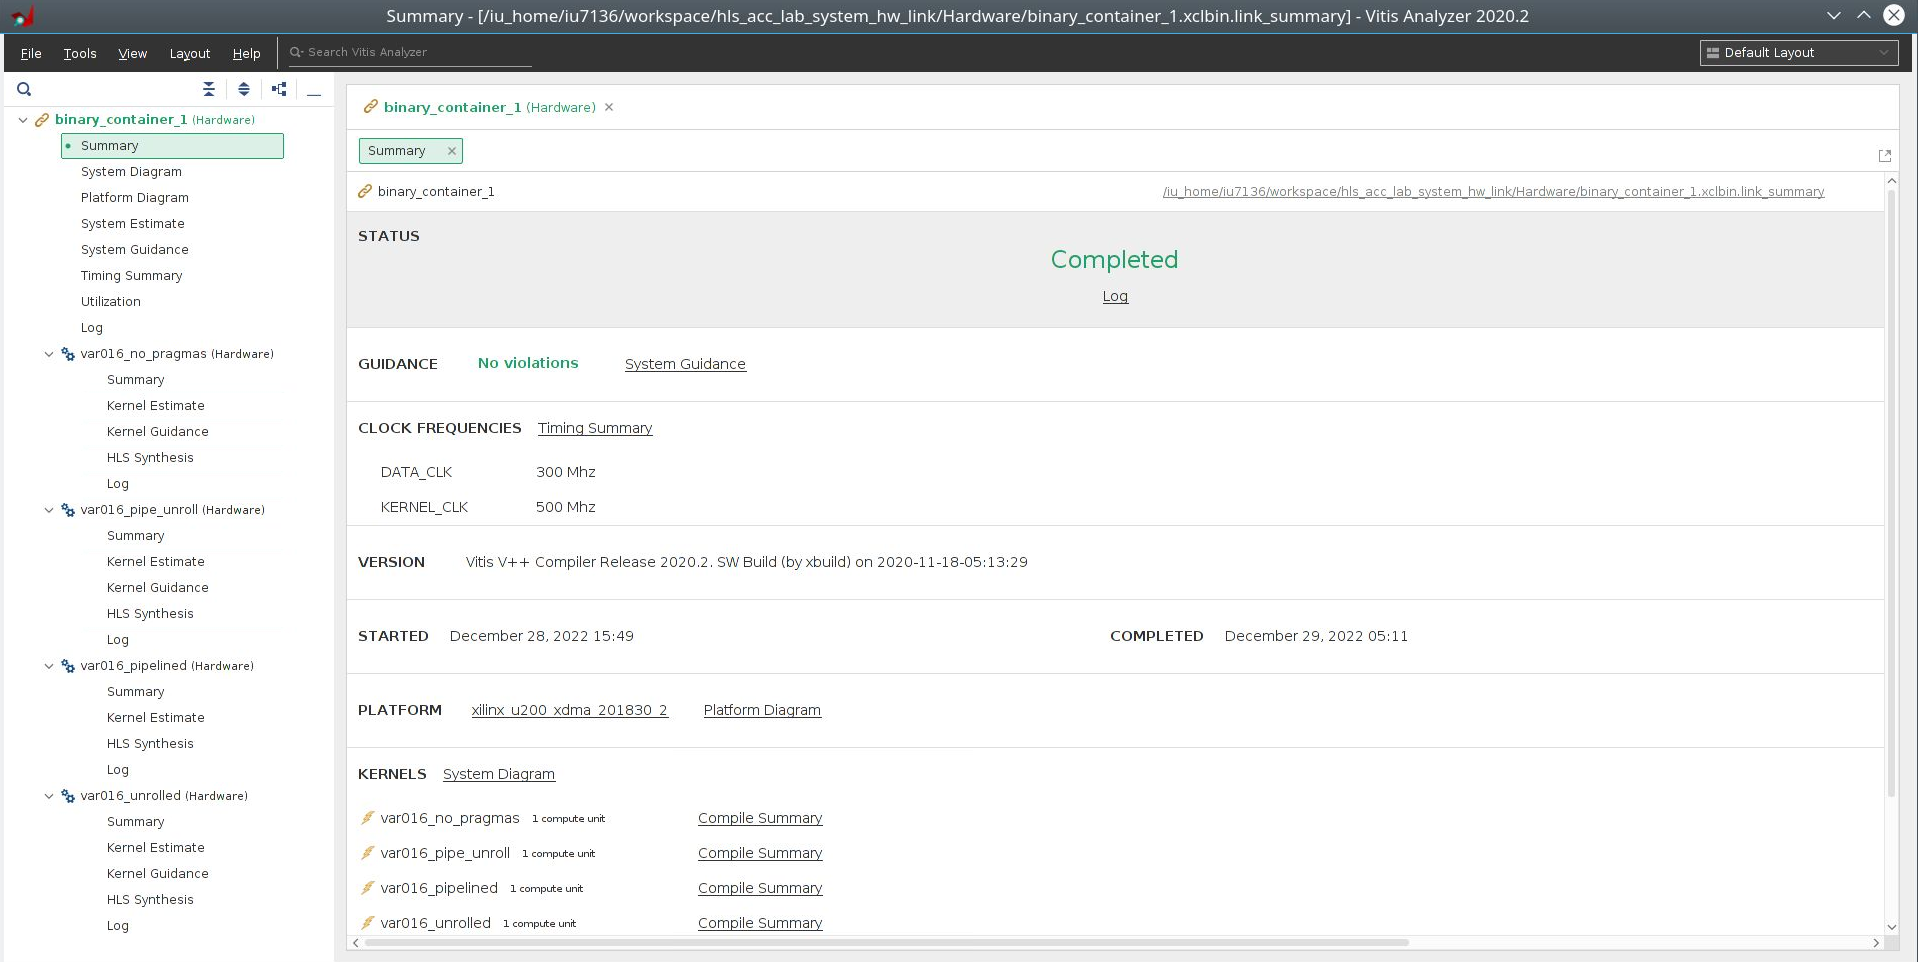
\includegraphics[scale=0.3]{images/hardware_1}
		\caption{Копия экрана вкладки "Summary"}
		\label{png:summary}
	}
\end{figure}

На рисунке \ref{png:system} копия экрана вкладки "System Diagram".
\begin{figure}[H]
	\captionsetup{justification=centering}
	\centering{
		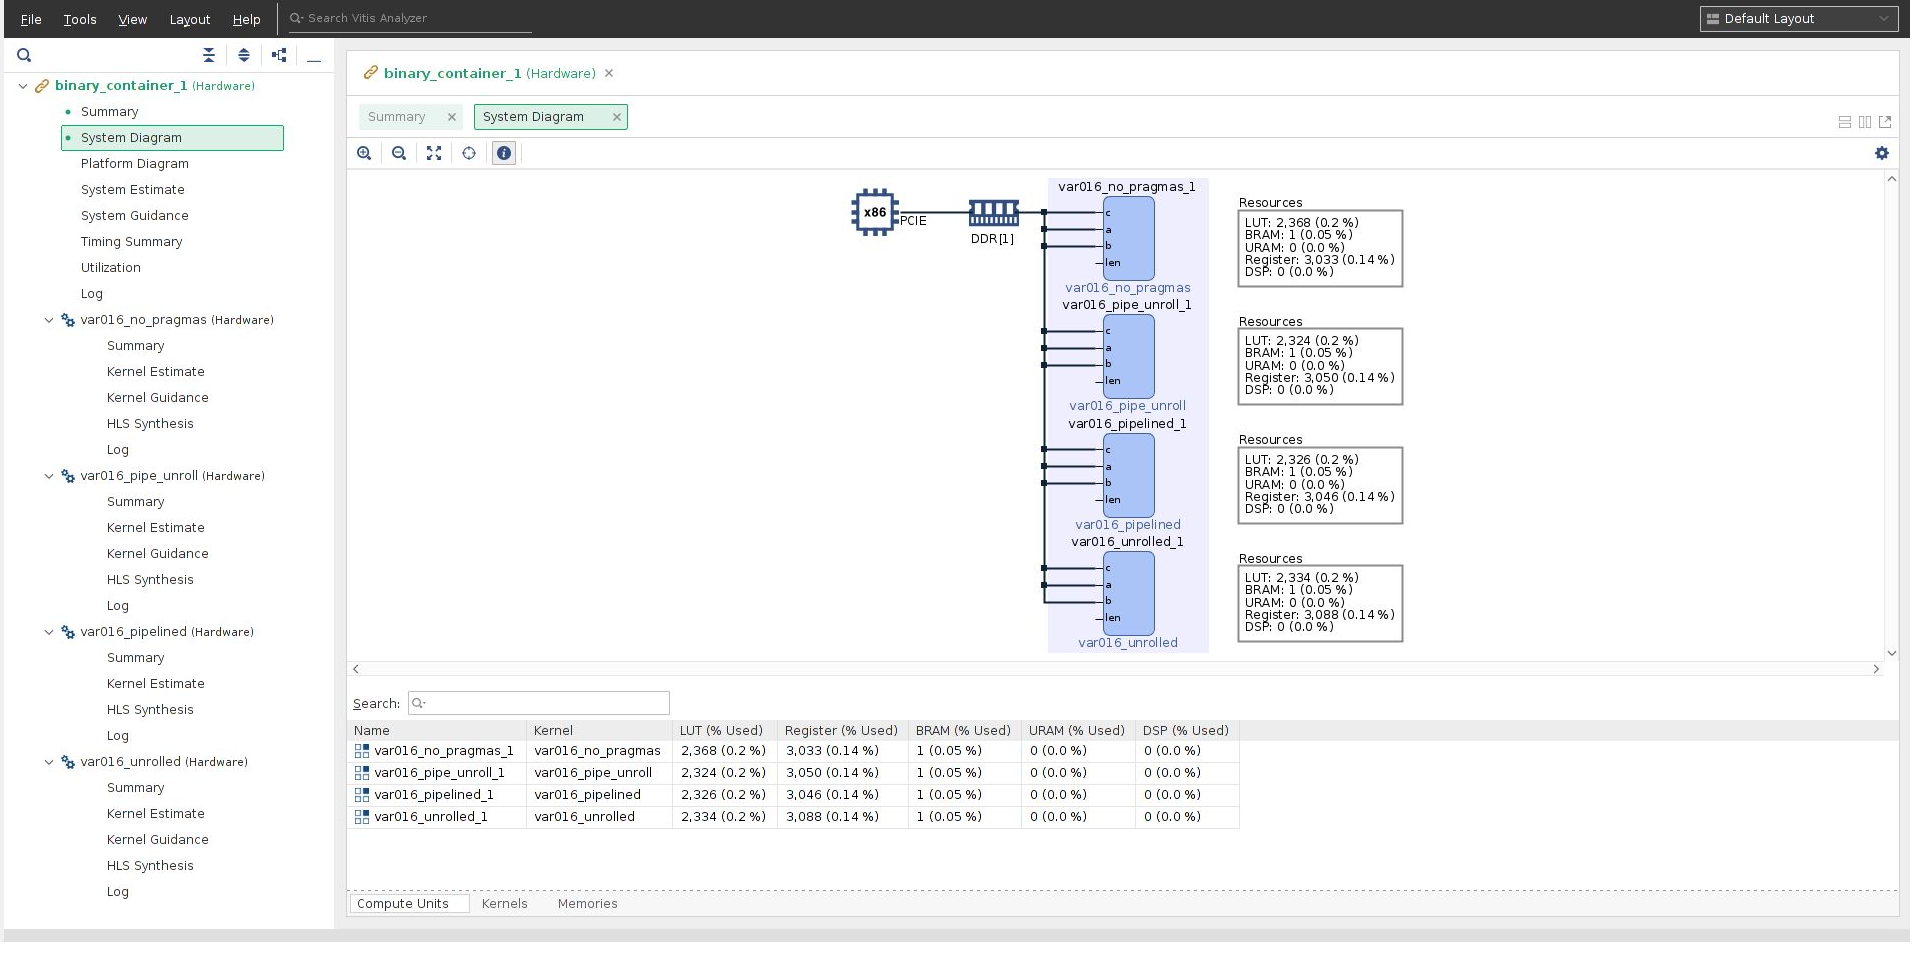
\includegraphics[scale=0.3]{images/hardware_2}
		\caption{Копия экрана вкладки "System Diagram"}
		\label{png:system}
	}
\end{figure}

На рисунке \ref{png:platform} копия экрана вкладки "Platform Diagram".
\begin{figure}[H]
	\captionsetup{justification=centering}
	\centering{
		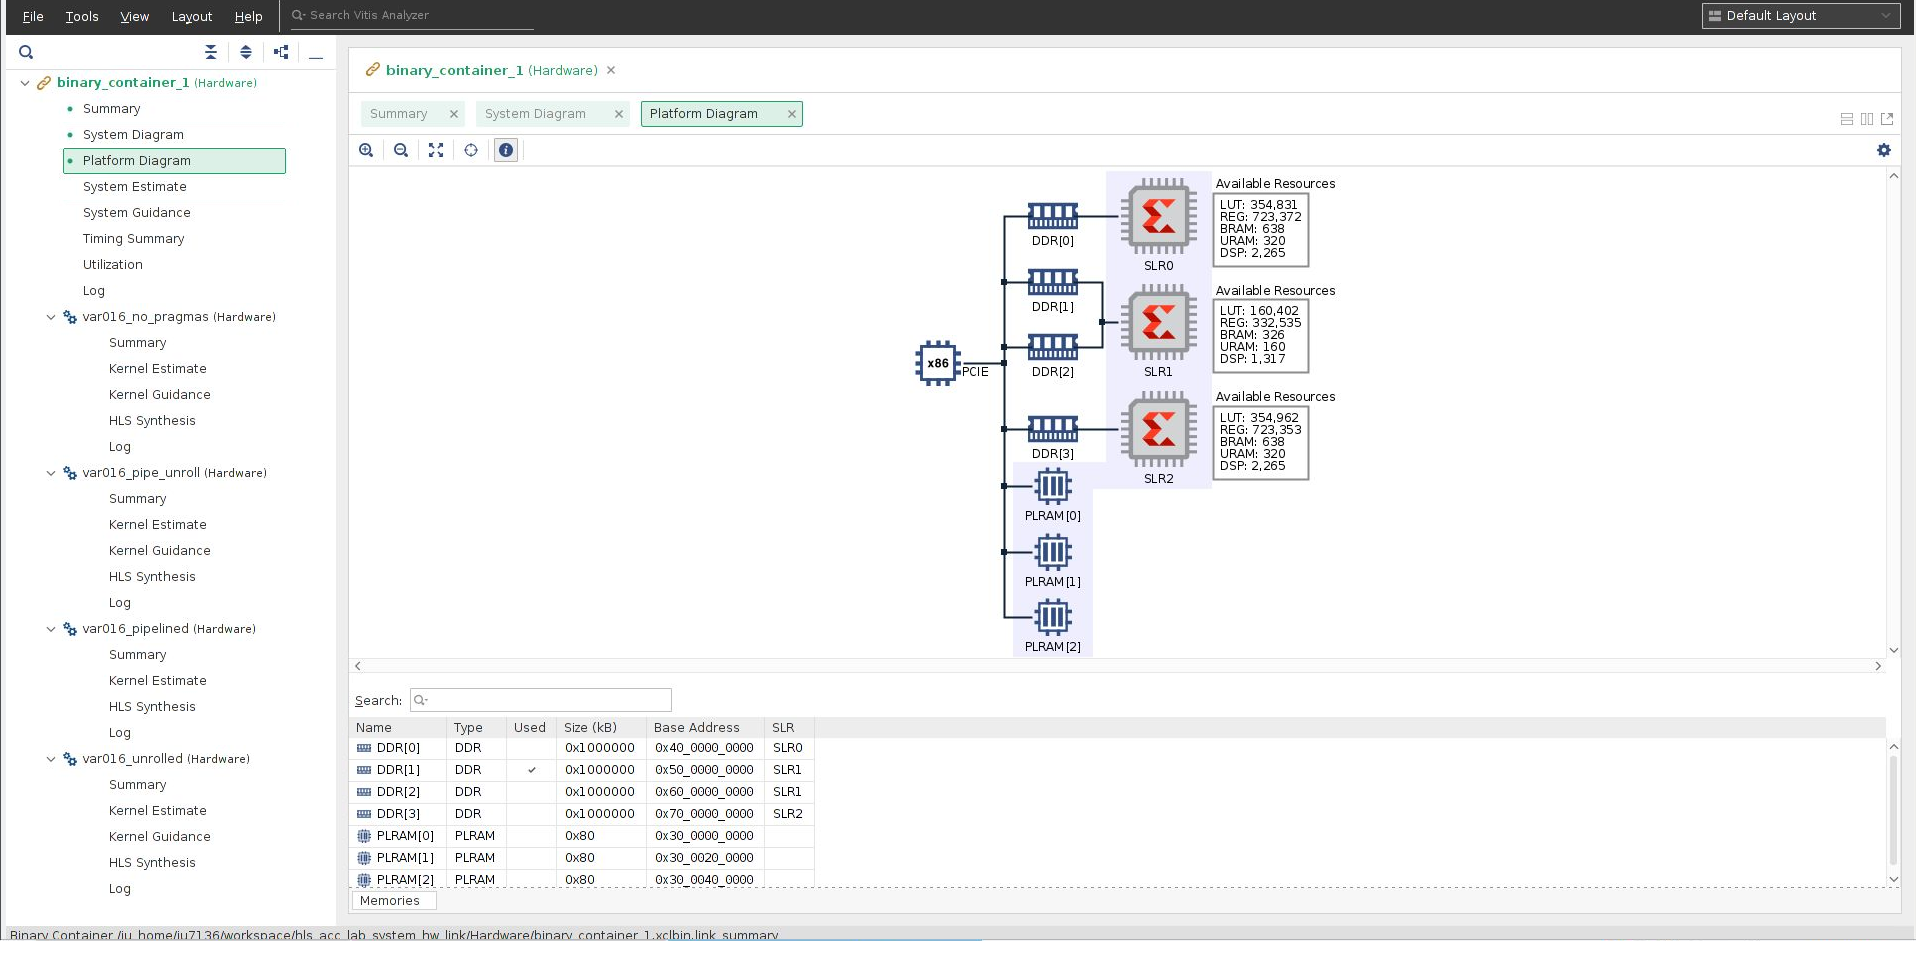
\includegraphics[scale=0.3]{images/hardware_3}
		\caption{Копия экрана вкладки "Platform Diagram"}
		\label{png:platform}
	}
\end{figure}

На рисунке \ref{png:hls_1} копия экрана вкладки "HLS Synthesis" для ядра "no\_pragmas".
\begin{figure}[H]
	\captionsetup{justification=centering}
	\centering{
		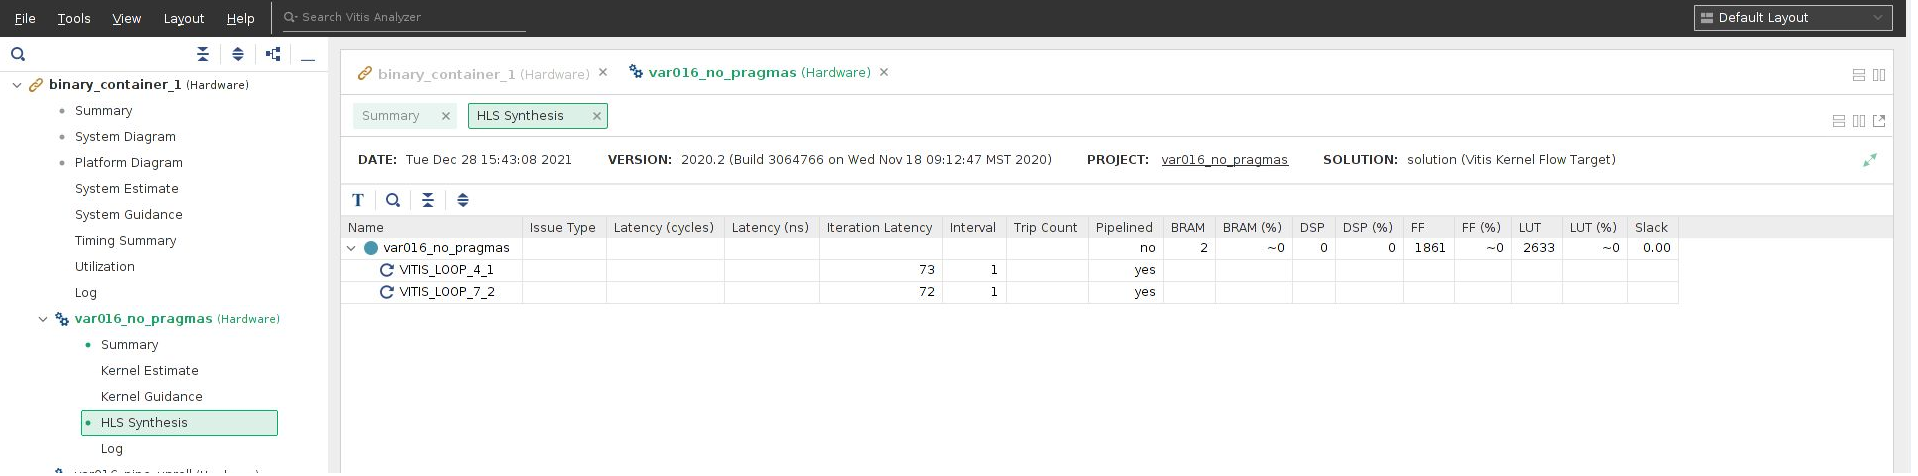
\includegraphics[scale=0.3]{images/hls_1}
		\caption{Копия экрана вкладки "HLS Synthesis" для ядра "no\_pragmas"}
		\label{png:hls_1}
	}
\end{figure}

На рисунке \ref{png:hls_2} копия экрана вкладки "HLS Synthesis" для ядра "pipe\_unroll".
\begin{figure}[H]
	\captionsetup{justification=centering}
	\centering{
		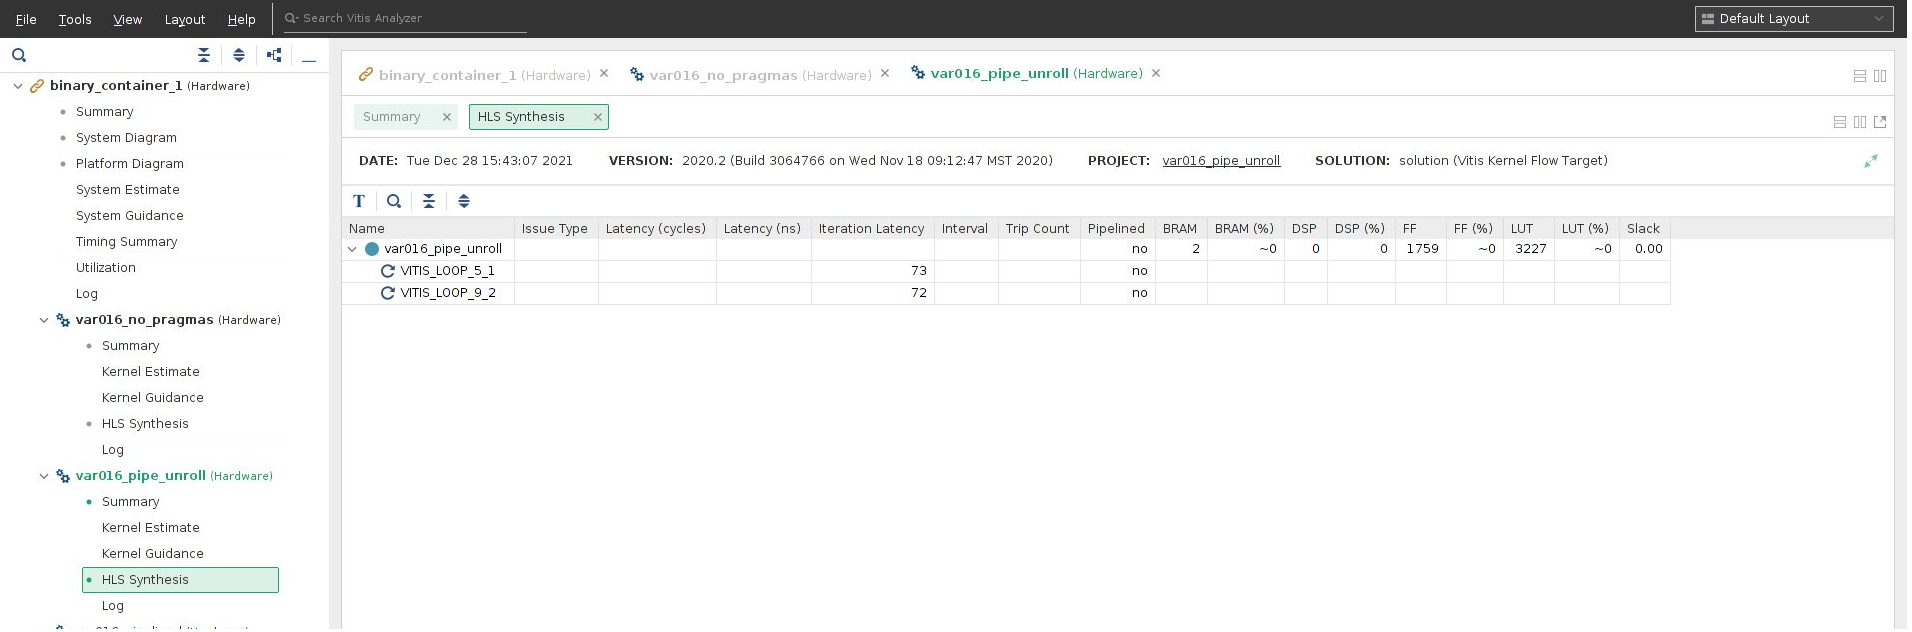
\includegraphics[scale=0.3]{images/hls_2}
		\caption{Копия экрана вкладки "HLS Synthesis" для ядра "pipe\_unroll"}
		\label{png:hls_2}
	}
\end{figure}

На рисунке \ref{png:hls_3} копия экрана вкладки "HLS Synthesis" для ядра "pipelined".
\begin{figure}[H]
	\captionsetup{justification=centering}
	\centering{
		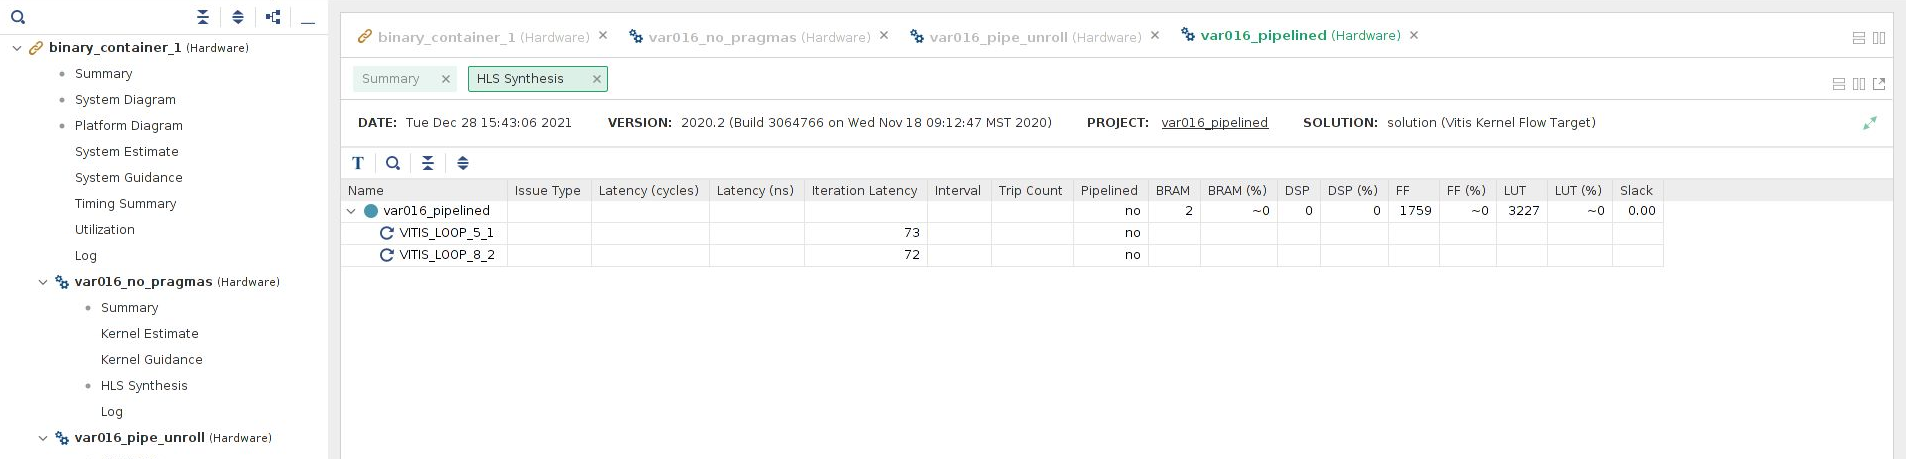
\includegraphics[scale=0.3]{images/hls_3}
		\caption{Копия экрана вкладки "HLS Synthesis" для ядра "pipelined"}
		\label{png:hls_3}
	}
\end{figure}


На рисунке \ref{png:hls_4} копия экрана вкладки "HLS Synthesis" для ядра "unrolled".
\begin{figure}[H]
	\captionsetup{justification=centering}
	\centering{
		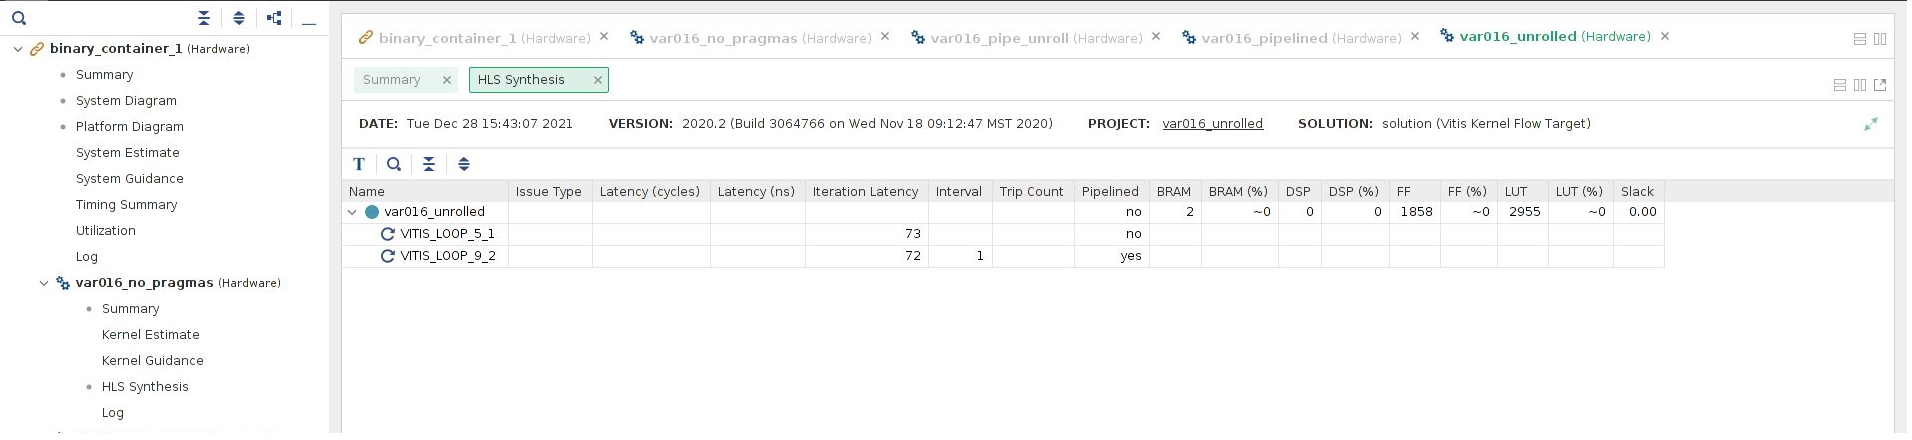
\includegraphics[scale=0.35]{images/hls_4}
		\caption{Копия экрана вкладки "HLS Synthesis" для ядра "unrolled"}
		\label{png:hls_4}
	}
\end{figure}



На рисунке \ref{png:hardware} представлен результат работы приложения в режиме Hardware.

\begin{figure}[H]
	\captionsetup{justification=centering}
	\centering{
		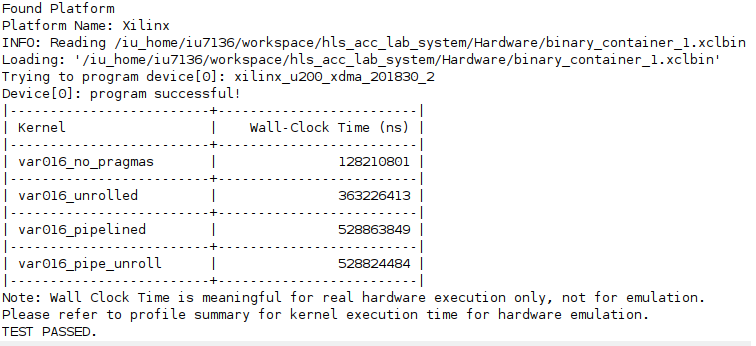
\includegraphics[scale=0.7]{images/hardware_result}
		\caption{Результаты работы приложения в режиме Hardware}
		\label{png:hardware}
	}
\end{figure}